\documentclass[11pt]{article}
\usepackage[margin=0.85in]{geometry}
\usepackage{enumitem}
\usepackage{tabularx}
\usepackage{amsmath}
\usepackage{amssymb}
\usepackage{tikz}
\usepackage{array}
\usepackage{titlesec}
\usepackage[most]{tcolorbox}
\usepackage{xcolor}

\definecolor{dayblue}{HTML}{2B5C8A}
\definecolor{tealheader}{HTML}{0097A7}
\definecolor{calloutgreen}{HTML}{D9EAD3}

\setlength{\parindent}{0pt}
\renewcommand{\arraystretch}{1.3}

\titleformat{\section}{\large\bfseries}{\thesection}{0.5em}{}

\newcommand{\framedline}[1]{\underline{\hspace{#1}}}
\newcommand{\frameblank}{\underline{\hspace{4em}}}
\newcommand{\sketchbox}[1]{%
  \begin{tikzpicture}
    \draw[thin,gray!50] (-3,-2) grid (3,2);
    \draw[->] (-3.2,0) -- (3.2,0) node[right] {\small $x$};
    \draw[->] (0,-2.2) -- (0,2.2) node[above] {\small $y$};
    \node at (0,-2.6) {\scriptsize #1};
  \end{tikzpicture}%
}

\begin{document}

\begin{center}
{\Large\bfseries Lesson 3-5, Day 3 --- Multiplicity \& Factored-Form Graphing} \\[2pt]
{\small Name: \framedline{2.5in} \quad Period: \framedline{0.5in} \quad Date: 5/8/26}
\end{center}

\vspace{0.5em}
\hrule
\vspace{0.5em}

%% ---- OBJECTIVES (three-row tcolorbox table, matches L41_P2 pattern) ----
\begin{tcolorbox}[
  enhanced,
  breakable,
  colback=calloutgreen,
  colframe=black!55,
  boxrule=0.7pt,
  arc=2pt,
  left=6pt, right=6pt, top=5pt, bottom=5pt
]
{\small
\renewcommand{\arraystretch}{1.4}
\noindent\begin{tabular}{|>{\bfseries}p{1.5in}|p{5.0in}|}
\hline
Math Objective & Construct a factored polynomial from a graph by identifying x-intercepts, choosing the correct multiplicity at each (touch = even, cross = odd), and applying end behavior to determine the leading coefficient sign. \\ \hline
Language Objective & Students will use the frame ``The factor for $x = $ \underline{\hspace{0.6em}} must be \underline{\hspace{0.6em}} because the graph \underline{\hspace{0.6em}}'' to justify each factor of a polynomial, and explain why even multiplicity produces a touch while odd multiplicity produces a cross. \\ \hline
Essential Understanding & A polynomial's graph and its factored form encode the same information --- zeros locate the factors, multiplicity determines the local behavior at each x-intercept (touch vs.\ cross), and end behavior determines the leading coefficient sign. \\ \hline
\end{tabular}
}
\end{tcolorbox}

\vspace{0.3em}

\textbf{Sentence frames (use these when you share):}
\begin{itemize}[leftmargin=*, nosep]
    \item ``The factor for $x = \frameblank$ must be \frameblank\ because the graph \frameblank.''
    \item ``The leading coefficient is \frameblank\ because the ends go \frameblank.''
    \item ``I notice \frameblank, so I think \frameblank.''
\end{itemize}

\vspace{0.5em}
\hrule

\section*{Do Now (5 min)}

\textit{Quick recall from yesterday.}

\begin{enumerate}[label=\textbf{\arabic*.}, leftmargin=*]
    \item What is the multiplicity of the zero $x = 4$ in $f(x) = (x-4)^2(x+1)$? \framedline{3in}
    \item If a zero has \textbf{even} multiplicity, what does the graph do at that zero?
    \par\hspace{2em} \framedline{5in}
    \par\hspace{2em} \framedline{5in}
    \item If a zero has \textbf{odd} multiplicity, what does the graph do at that zero?
    \par\hspace{2em} \framedline{5in}
    \par\hspace{2em} \framedline{5in}
\end{enumerate}

\vspace{0.5em}
\hrule

\section*{Launch (15 min) --- Gradual release}

\subsection*{I do (4 min): watch and annotate}

Teacher example: $f(x) = (x-2)^2(x+3)$.

Annotate the example as the teacher works through it. Write what each piece tells you:

\begin{tabularx}{\textwidth}{|>{\bfseries}l|X|}
\hline
Zero $x = 2$ & multiplicity = \frameblank, \quad behavior at zero: \framedline{3in} \\[6pt]
\hline
Zero $x = -3$ & multiplicity = \frameblank, \quad behavior at zero: \framedline{3in} \\[6pt]
\hline
Degree & \frameblank, \quad leading coefficient sign: \framedline{2in} \\[6pt]
\hline
End behavior (left, right) & \framedline{2.5in}, \framedline{2.5in} \\[6pt]
\hline
\end{tabularx}

\vspace{0.5em}
\textbf{Touch / Cross rule (write what the teacher says):} \\
\framedline{6in} \\[8pt]
\framedline{6in} \\[8pt]
\framedline{6in}

%% ---- YOU DO + GRID: kept on the same page ----
\begin{samepage}
\subsection*{You do (4 min): try this one yourself}

\textbf{Sketch} $g(x) = (x+1)(x-4)^2$ on the grid below. Label both zeros and indicate which is a touch and which is a cross.

\begin{center}
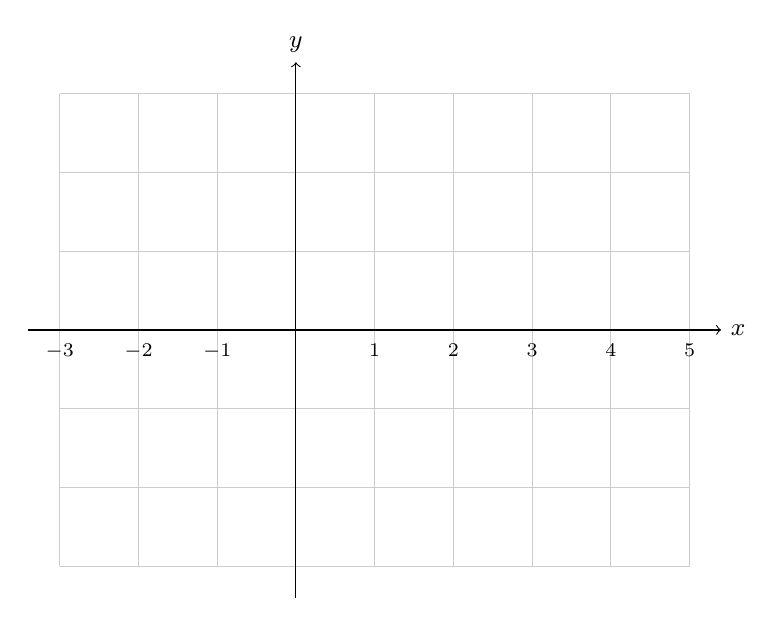
\begin{tikzpicture}
  \draw[thin,gray!40] (-3,-3) grid (5,3);
  \draw[->] (-3.4,0) -- (5.4,0) node[right] {\small $x$};
  \draw[->] (0,-3.4) -- (0,3.4) node[above] {\small $y$};
  \foreach \x in {-3,-2,-1,1,2,3,4,5} \node[below,font=\scriptsize] at (\x,-0.05) {$\x$};
\end{tikzpicture}
\end{center}

\textbf{Why?} \framedline{5.5in} \\[8pt]
\framedline{6in} \\[8pt]
\framedline{6in}
\end{samepage}

\subsection*{I check (3 min)}

Compare your sketch with the projected exemplar. \textbf{What did you fix?} \\
\framedline{5in} \\[6pt]
\framedline{5in}

\subsection*{We do together (4 min)}

Class example: $h(x) = -x(x+2)^2(x-1)$. Fill in as we go.

\begin{itemize}[leftmargin=*, nosep]
    \item Zeros: $x = $ \frameblank, \frameblank, \frameblank
    \item Touch or cross at each? \framedline{5in}
    \item End behavior: left \frameblank, right \frameblank \quad (Why? \framedline{3in})
\end{itemize}

\vspace{0.5em}
\hrule

\section*{Explore (25 min)}

\subsection*{Mystery Graph (10 min, think-pair-share) --- DOK 3}

The graph below has zeros at $x = -1$ (touch) and $x = 3$ (cross). \textbf{Both ends point downward.}

\begin{center}
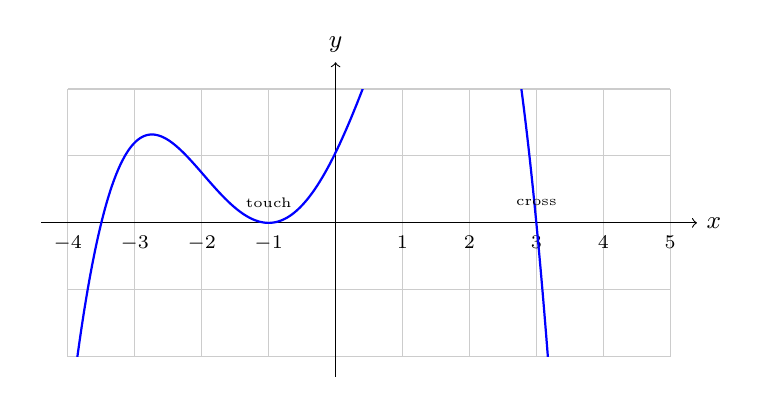
\begin{tikzpicture}[scale=0.85]
  % Grid and axes — y clipped to [-2, 2]
  \draw[thin,gray!40] (-4,-2) grid (5,2);
  \draw[->] (-4.4,0) -- (5.4,0) node[right] {\small $x$};
  \draw[->] (0,-2.3) -- (0,2.4) node[above] {\small $y$};
  \foreach \x in {-4,-3,-2,-1,1,2,3,4,5} \node[below,font=\scriptsize] at (\x,-0.05) {$\x$};
  % Clip curve to the grid rectangle so it never exits the box
  \begin{scope}
    \clip (-4,-2) rectangle (5,2);
    \draw[thick, blue, domain=-4:5, samples=300, smooth]
      plot (\x, {-0.10*(\x+1)*(\x+1)*(\x-3)*(\x+3.5)});
  \end{scope}
  \node[font=\tiny] at (-1,0.3) {touch};
  \node[font=\tiny] at (3,0.3) {cross};
  % Explicit bounding box — prevents TikZ from auto-expanding beyond the grid
  \path[use as bounding box] (-4.6,-2.5) rectangle (5.6,2.6);
\end{tikzpicture}
\end{center}

\textit{(Note: this graph has more than two zeros --- you only need to account for the two labeled. Focus on what those two tell you about factors and what the ends-down behavior tells you about leading coefficient and degree.)}

\vspace{0.5em}
\textbf{Build a possible factored form for this graph. Justify every piece.}

\textbf{My factored form:} $f(x) = $ \framedline{4.5in}

\vspace{4pt}
\textbf{Why this factor for $x = -1$?} \\
\framedline{5.5in} \\[8pt]
\framedline{5.5in}

\vspace{4pt}
\textbf{Why this factor for $x = 3$?} \\
\framedline{5.5in} \\[8pt]
\framedline{5.5in}

\vspace{4pt}
\textbf{Why this leading coefficient?} \\
\framedline{5.5in} \\[8pt]
\framedline{5.5in}

\vspace{4pt}
\textbf{Could the degree be different and still match?} \\
\framedline{5.5in} \\[8pt]
\framedline{5.5in}

\subsection*{DOK-2 consolidation items (15 min, partners)}

\textbf{1. (Savvas q12)} Sketch the graph of $f(x) = 3x^3 - 9x^2 - 12x$ by first finding its zeros.

\textbf{Factored form:} $f(x) = $ \framedline{4in}

\vspace{4pt}
\textbf{Zeros:} \framedline{4in}

\begin{center}
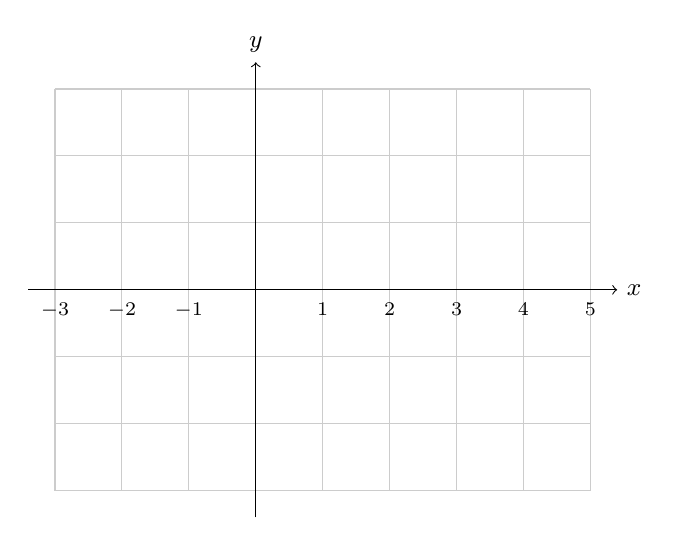
\begin{tikzpicture}[scale=0.85]
  \draw[thin,gray!40] (-3,-3) grid (5,3);
  \draw[->] (-3.4,0) -- (5.4,0) node[right] {\small $x$};
  \draw[->] (0,-3.4) -- (0,3.4) node[above] {\small $y$};
  \foreach \x in {-3,-2,-1,1,2,3,4,5} \node[below,font=\scriptsize] at (\x,-0.05) {$\x$};
\end{tikzpicture}
\end{center}

\vspace{0.5em}

\textbf{2. (Try-It 2b)} Describe the behavior of the graph of $f(x) = (x^2 + 9)(x - 1)^5(x + 2)^2$ at each of its zeros.

\begin{itemize}[leftmargin=*, nosep]
    \item Real zeros: \framedline{4in}
    \item At $x = 1$: multiplicity \frameblank, \quad touch / cross? \framedline{2.5in}
    \item At $x = -2$: multiplicity \frameblank, \quad touch / cross? \framedline{2.5in}
    \item What about the factor $(x^2 + 9)$? \\
    \framedline{5.5in} \\[6pt]
    \framedline{5.5in}
\end{itemize}

\vspace{0.5em}

\textbf{3.} A polynomial graph crosses at $x = 0$, touches at $x = 2$, and both ends point upward.

\textbf{Write a possible factored form:} $f(x) = $ \framedline{4in}

\vspace{4pt}
\textbf{Justify the leading coefficient sign:} \\
\framedline{5.5in} \\[8pt]
\framedline{5.5in}

\vspace{0.5em}
\hrule

\section*{Share / Summary (5 min)}

\textbf{Today's rule, in your words:} \\
\framedline{6in} \\[8pt]
\framedline{6in}

\textbf{One way the rule helped me on items 1--3 today:} \\
\framedline{6in} \\[8pt]
\framedline{6in}

\vspace{0.5em}
\hrule

\section*{Exit Ticket (5 min)}

\begin{enumerate}[label=\textbf{\arabic*.}, leftmargin=*]
    \item A factor of $(x-4)^2$ produces a \framedline{2in} at $x = 4$. \quad (touch / cross)
    \item A factor of $(x+1)$ produces a \framedline{2in} at $x = -1$. \quad (touch / cross)
    \item \textbf{The biggest thing I learned today was:} \\
        \framedline{6in} \\[8pt]
        \framedline{6in}
\end{enumerate}

\end{document}
